% main introduction
\chapter{Introduction}
\label{ch:intro}

In this first introduction Chapter contains all the necessary background information as well as an overview for the work discussed in this thesis. It summarised basic biological properties of DNA and cell biology as well as the respective technologies to read and analyse and evaluate the output of these methods.
\hyperref[intro-sec:DNA]{Section~\ref*{intro-sec:DNA}} delineates the role DNA plays for the cell and then \hyperref[intro-sec:ctDNA]{section~\ref{intro-sec:ctDNA}} shows how these standards are changed in the tumour and cell free context. \hyperref[intro-sec:sequencing]{Section~\ref{intro-sec:sequencing}} introduces the current technologies used to measure and detect DNA and its variations. With \hyperref[intro-sec:somatic]{section~\ref*{intro-sec:somatic}} covering the computational analysis methods to read out changes in the DNA. Then \hyperref[intro-sec:lungcancer]{section~\ref{intro-sec:lungcancer}} relates how these changes lead to cancer and what we can learn from them. 
The introduction concludes with \hyperref[intro-sec:overview]{section~\ref*{intro-sec:overview}} as an overview over the thesis aims and my work in addressing them in the following chapters.


%%% this just contains all the links and possible formating of the introduction as a whole

% background of DNA
\section[DNA]{DNA as a information storage unit}
\label{intro-sec:DNA}
It is a widely accepted fact, that Deoxyribonucleic acid (DNA) serves as the long term information storage molecule of our cells. This information is protected and allows correction of simple errors through its double helix structure \cite{Watson1953,Liang1998}. The nucleotides, which consist of a deoxyribose sugar (hence the name), a phosphate group and the nitrogenous base, are joined together by phosphate groups. Even though there are six common naturally occurring nitrogenous bases: adenine (A), thymine (T), guanine (G), cytosine (C), uracil (U) and nicotinamide, only the first four are used to encode the genetic information into DNA. Each of the strands mirrors the other, so that an adenine will be paired up with a thymine forming two hydrogen bonds. Similarly cytosine will pair with guanine forming an even stronger bond with three hydrogen bonds. While other pairings which do not follow those rules are chemically possible, they are mostly observed in ribonucleic acid (RNA) \cite{Sinden1994}. These very strict bonding rules enable the DNA to be similar to a hard drive with backup on a computer. And as only one strand contains all the information, the DNA polymerase enzyme does only need access to one strand, which allows parallel replication during cell division, but also error corrections, by proof reading the newly synthesised strand with the template.
The DNA in eukaryotes however is not free floating around in the nucleus of a cell, but rather it is highly organised around histones, which then form something resembling a spool of thread. This allows some of the DNA to be accessible where the use of other areas can be restricted. Through this restriction, the availability of certain genes, which are the sections of the DNA, which encode for short term storage molecules like RNA. This restriction plays an important role in cell fate and cell viability. Ultimately all information stored to create a new highly complex organism is stored in just the DNA of one cell. Whichever parts are used and how they are used decides the function and the identity of the cell.
\subsection[Mutations]{Phantastical mutations and where to find them}
However even though the DNA is highly stable and error correction methods are constantly working to not introduce any changes in the DNA, the source of evolution and adaptation of species is sourced in a steady mutation rate. These changes in normal tissue are mostly irrelevant to the organism as a whole and will not be passed on to the next generation. These changes are known as somatic mutations. This type of mutation accumulates in a cell linearly over the course of the lifespan of the cell and is not bound to just cell divisions\cite{Alexandrov2015,Moore2021}. 
In contrast, if one of those mutations occurs in the germline cell, eg. sperm or egg producing cells, these mutations will be propagated to all offspring and be present in all cells of that organism and in term all its offspring. These mutations are called germline mutations. These mutations are also called germline variants, as they establish in the population and represent a variation of the organism.

% background of ctDNA
\section[cfDNA]{Cell free DNA is more than just bits and pieces}
\label{intro-sec:ctDNA}

When a cell from a multicellular organism dies, through which ever method, there will be numerous enzymes involved, which clear the debris and recycle material. This means that proteases digest proteins into amino acids, which will later be used for either building new proteins or possibly even digested further for energy production. The same happens with the DNA in the cell when it is released following cell death. However, as discussed in the previous section~\ref{intro-sec:DNA} the DNA is wrapped around histones and organised in structures called nucleosomes. These protect the DNA from being cut by DNAases by hindering the access to the DNA, similar to how they stopped the access for transcription into RNA. This then in turn leads to the DNA being cut in the linker regions between nucleosomes into fragments mainly in the length of 167 base pairs (bp). 

These DNA fragments, which are called cell free DNA (cfDNA), can then be readily detected in bodily fluids, like blood, urine or even stool. By analysing these fragments, non invasive tests for prenatal care have been made possible, as the DNA of the developing foetus can be detected in the mother's blood \cite{Dan2012,Nicolaides2013}.

Similar to this process, a cancer also sheds DNA, titled ``circulating tumour DNA`` (ctDNA), when its cells die, either through intervention of the immune system, cancer therapies or other processes. These ctDNA fragments can similarly be analysed and molecular properties measured, without even knowing the exact location of the tumour. As a blood test can be routinely performed in the clinic, the monitoring of cancer progression is significantly easier and safer than through other measures. Of course, it is, similar to the prenatal test, acting as a proxy for the cells which are still alive, which have have not yet shed their DNA. Additionally, the amount of shedded DNA is highly variable between tumours, with a general higher amount seen in later stages when tumour burden is high \cite{Diehl2008,Schwarzenbach2011}.

\begin{figure}[hbt]
\centering
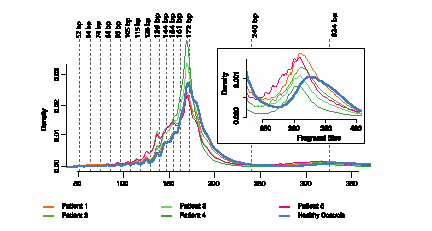
\includegraphics[width=0.9\linewidth]{Figures/intro/fragmentSizeDist}
\caption[Fragment size distribution of ctDNA]{Fragment size distribution of 5 high grade serous
ovarian carcinoma (HGSOC) patients and panel of healthy controls. The vertical dashed lines are placed on the fragment sizes between 52 and 172 bp where 10 bp periodicity is observed. The vertical lines at 240 and 324 bp show the range at which a shift in the di-nucleosomal peak occurs between HGSOC patients and healthy controls. The inset plot enlarges the density profile in the di-nucleosomal fragment length range. Figure adopted from \textcite{Markus2022}}\label{fig:ctdnaFragSize}
\end{figure}

Due to the different biological processes which can lead to the release of DNA from cancer cells, in addition to apoptosis, which is the main source of cfDNA from healthy cells, ctDNA has several biological differences to cfDNA. The most prominent features observed are distinct ctDNA fragmentation size patterns, fragment start sites, and fragment ends motives. While the preferred end motive and start site are heavily correlated, restricting the analysis to the lower tail of the mono- and di-nuclesomal peak of the fragment size distribution (74-155bp and 240-325bp) allowed a ctDNA tumour signal enrichment of at least 28\%. This is enrichment and the high periodicity of the distribution showed a high dependence on nucleosomal placement. All ctDNA features combined were shown to be able to predict the presence or absence of tumour DNA in a samples regardless of tumour type  (\autoref{fig:ctdnaFragSize}, \cite{Mouliere2018,Markus2022}). 


% background of sequencing DNA
\section[DNA sequencing]{DNA sequencing - when is next generation sequencing the current generation?}
\label{intro-sec:sequencing}

As we know the building blocks, that make DNA as well as the process and the enzymes responsible, we can synthesise DNA in vitro. By chemically modifying the nucleotides supplied to the synthesis process, the sequence of the copied strand can be analysed. The first method to make use of this used the lambda phage to fuse known ends for the primers needed for the reaction to the piece of DNA and supplied labelled nucleotides \cite{Padmanabhan1974}.This method was then superseded by "Sanger sequencing" after Frederick Sanger who with colleagues published this method in 1977, by adding \textbf{di}deoxynucleotides in a low concentration, the polymerase chain reaction would terminate trying to integrate these nucleotides and by labelling them radioactively or flourecently, a gel can be used to determine the sequence of a piece of DNA\cite{Sanger1975,Sanger1977}, which made the method better suited for larger scale projects.

However this method has multiple issues for modern research questions. Mostly, that it is fairly labour and time consuming to analyse multiple pieces of DNA at the same time and it is very challenging to sequence all the DNA of an organism. The human genome project, which was started in 1990 used machines which automated the Sanger sequencing procedure and it still took hundreds of researchers 13 years to complete the DNA sequence of just one human \cite{Lander2001,Venter2001}. Even though this was a very long project, it laid the ground work for the usage of the current sequencing technologies.

\subsection[Library preparation]{Library preparation - what we learned from using phages}
\label{intro-sec:libraryprep}

\begin{figure}[!ht]
\centering
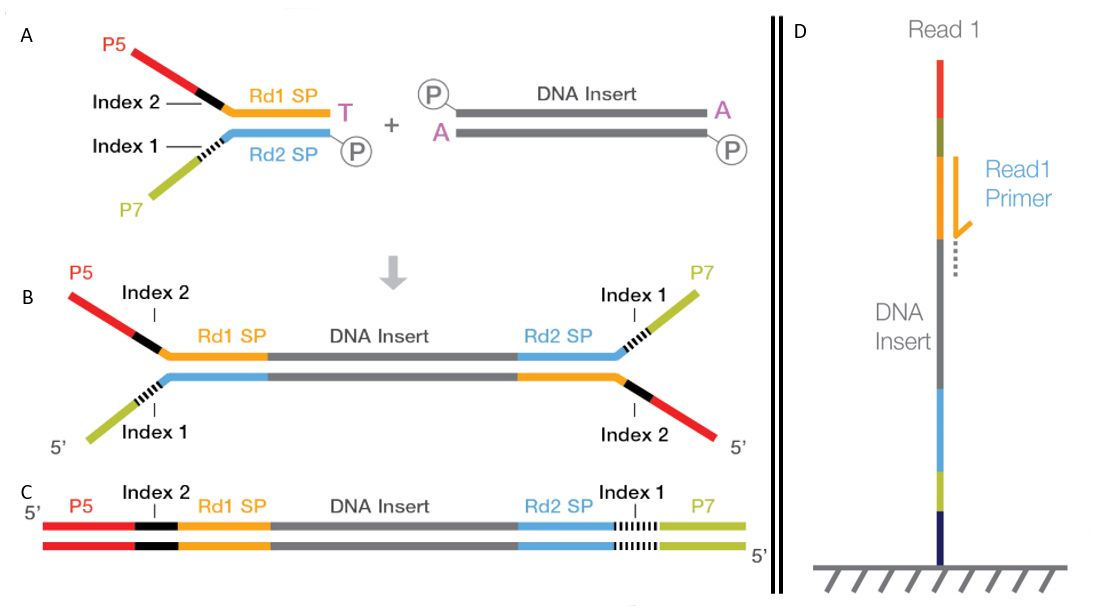
\includegraphics[width=.9\linewidth]{Figures/LibraryPreparation.png}
\caption[Library preparation for NGS]{Adapter ligation during library preparation. The adapters are added to the DNA insert during library preparation. A. The DNA insert is prepared by adding an A-tail and phosphorylation. B. The adapter complex which includes the P5/P7 flow cell binding adapter is added to the DNA insert. C. The DNA insert is ready for sequencing. D. The DNA insert binds to the flow cell for sequencing. Primers bind to the DNA insert to generate reads; \\Figure adapted from \href{https://sapac.support.illumina.com/bulletins/2020/12/how-short-inserts-affect-sequencing-performance.html}{"How short inserts affect sequencing performance"}\protect\cite{Illumina2020}}\label{fig:libraryprep}
\end{figure}

Library preparation is the name of the preprocessing step, which is done before it is sequenced with the current technologies. The first step to sequence DNA is to obtain the DNA, which is done by lysing the cells of interest, which disrupts the cell membrane and therefore spills all its contents. The then spilled DNA is fragmented into smaller pieces, by either restriction enzymes or sonication, to have a size of about between 200-800bp. These steps are not necessary when preparing sequencing of ctDNA, as discussed in \autoref{intro-sec:ctDNA}, the DNA is unbound and already digested into short fragments.
Once the DNA is ready, it is both phosphorelated as well as an A-tail is added, before the adapter complex is ligated. This enabled the DNA to bind to the flow cell which is covered with the reverse complement of the adapter \autoref{fig:libraryprep}. 

\subsection{Next generation sequencing}
\label{intro-sec:ngs}

\begin{figure}[!ht]
\centering
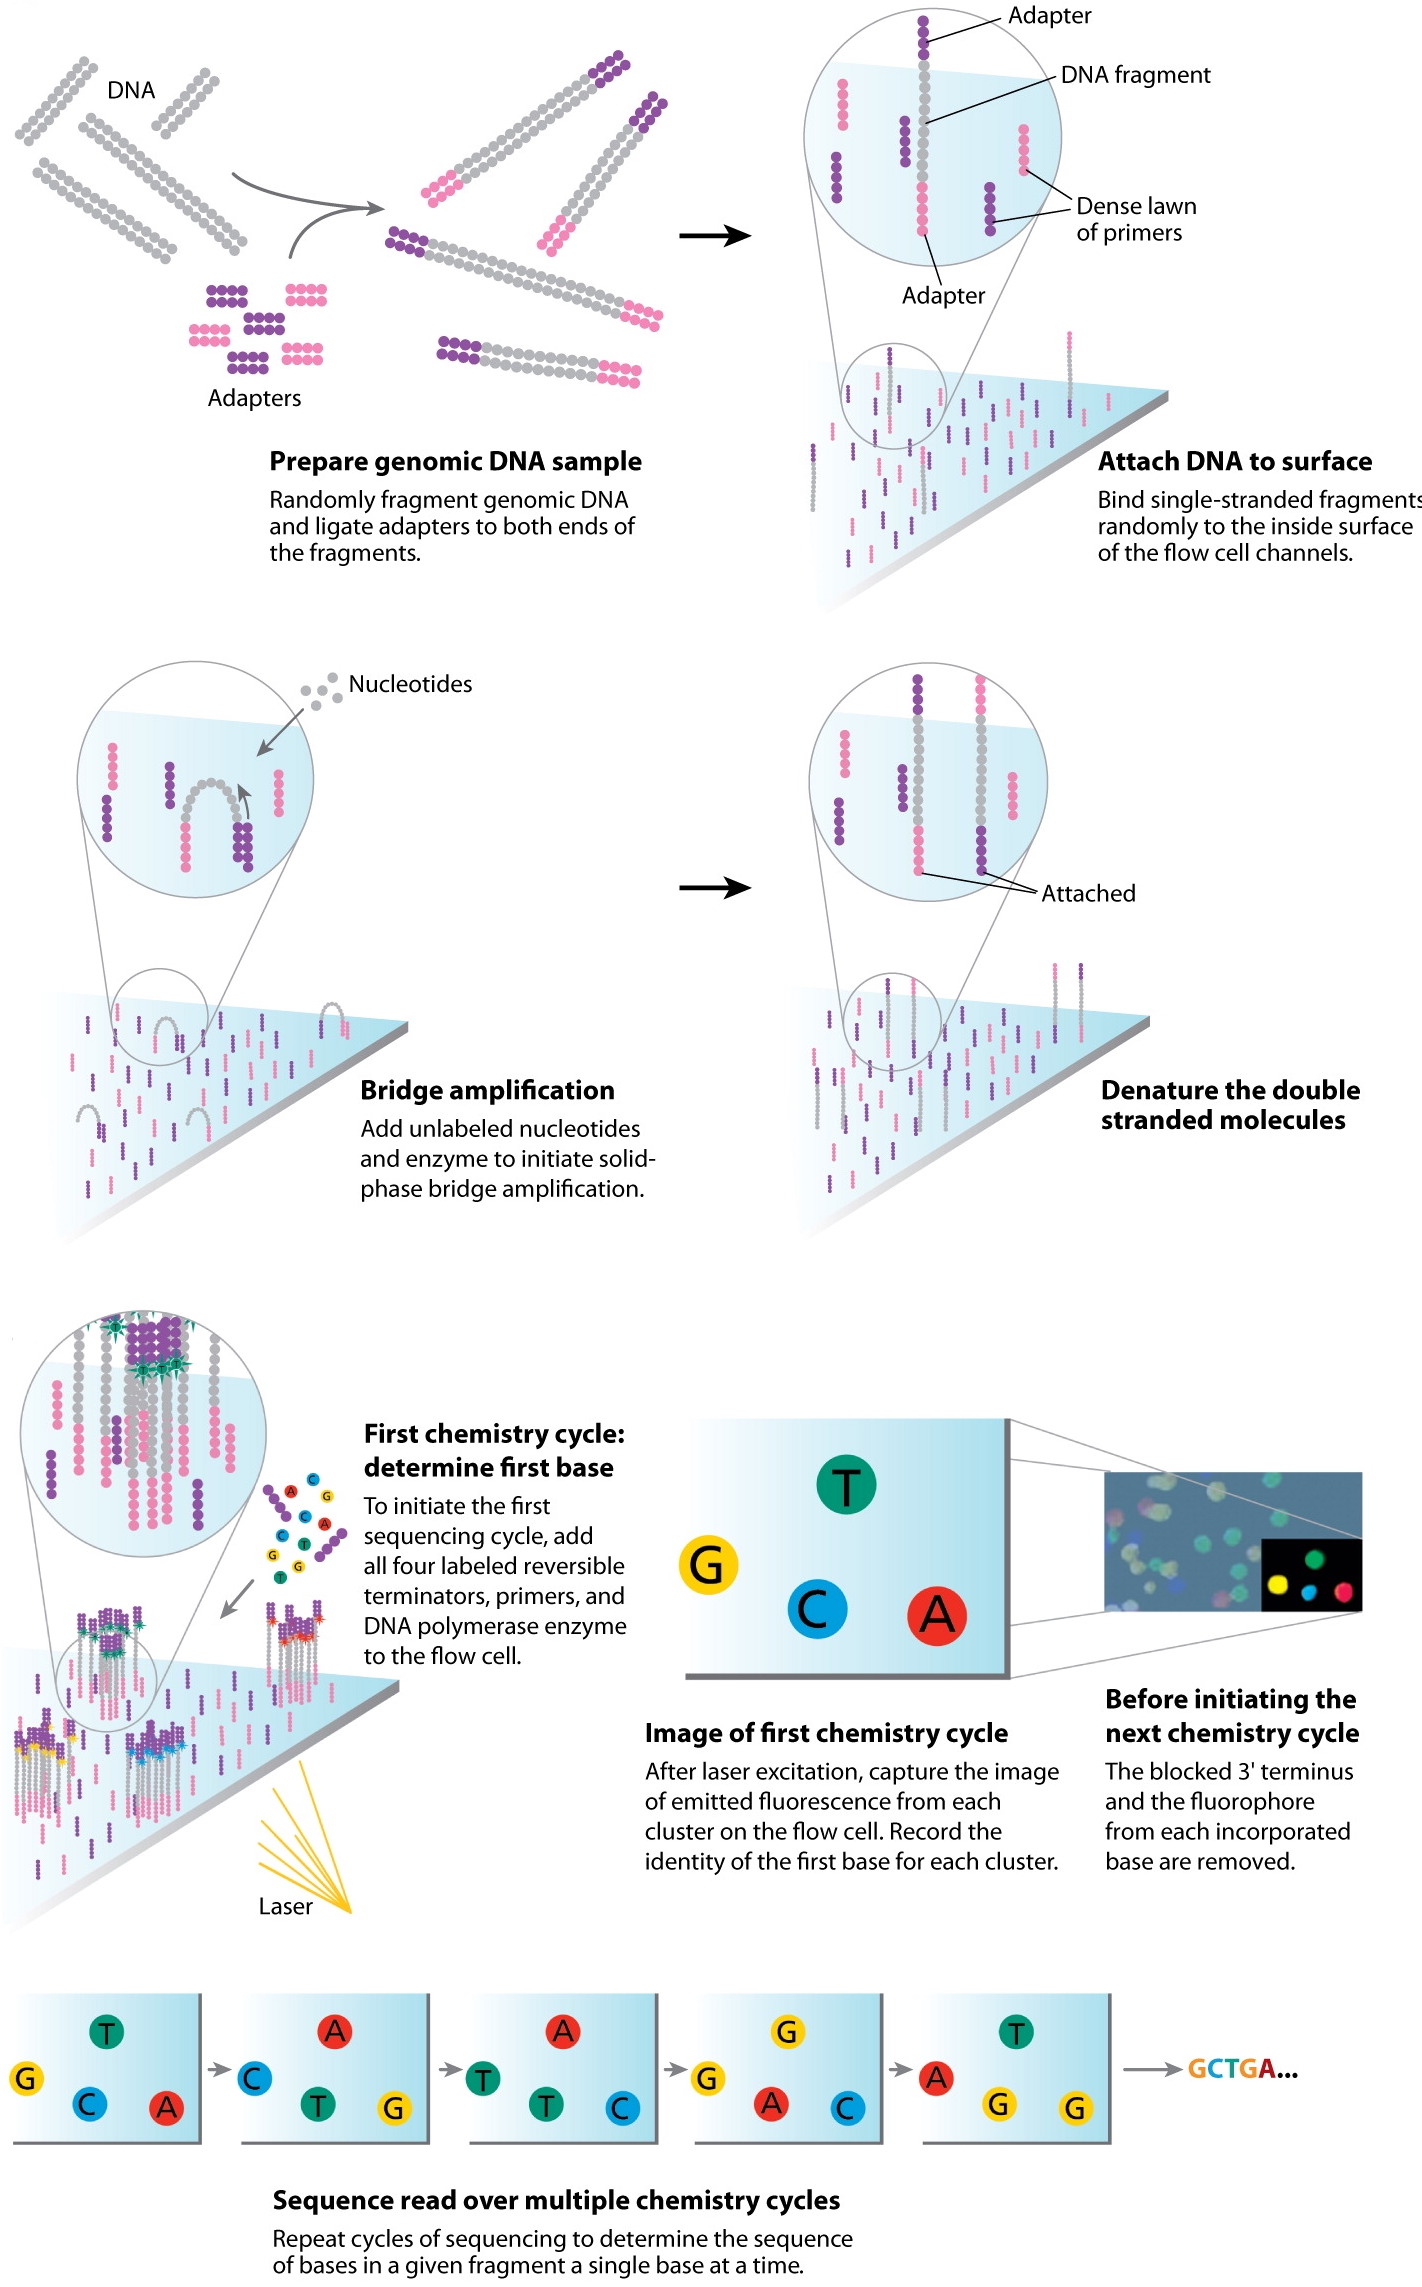
\includegraphics[width=.85\linewidth]{Figures/SequencingBySynthesis.jpg}
\caption[Sequencing by synthesis (Illumina)]{The Illumina sequencing-by-synthesis approach. Cluster strands created by bridge amplification are primed and all four fluorescently labeled, 3'-OH blocked nucleotides are added to the flow cell with DNA polymerase. The cluster strands are extended by one nucleotide. Following the incorporation step, the unused nucleotides and DNA polymerase molecules are washed away, a scan buffer is added to the flow cell, and the optics system scans each lane of the flow cell by imaging units called tiles. Once imaging is completed, chemicals that effect cleavage of the fluorescent labels and the 3'-OH blocking groups are added to the flow cell, which prepares the cluster strands for another round of fluorescent nucleotide incorporation; Figure adapted from \protect\citeauthor*{Mardis2008}\protect\cite{Mardis2008}}\label{fig:sequencingbysynthesis}
\end{figure}
%make sure the image comes as early as possible
\afterpage{\clearpage}

Next generation sequencing (NGS)is the coined term for basically any standard high-throughput sequencing performed, which includes exome, genome, transcriptome, protein-dna interactions (ChIP) and other epigenome studies. The term NGS is still widely used, even though it has been more than 10 years since the first NGS approach was commercially available. While in the beginning of next generation sequencing there were multiple approaches, the current lion share (80\% of sequencing data) of protocols use the Illumina short read sequencing by synthesis approach (\autoref{fig:sequencingbysynthesis})\cite{Mardis2008,Straiton2019}, which is based on the concept of alternating integration of florescently labelled nucleotides and imaging with a microscope (\autoref{fig:sequencingbysynthesis}) as well as multiplexing, where a DNA fragment is ligated to an index, which allows the sequencing of multiple samples at once \cite{Church1984,Church1988} as it is shown in \autoref{fig:libraryprep}. This method allows highly accurate determination of the sequence of a DNA fragment and depending on the flow cell and sequencing machine allows to sequence a whole genome in just 24h.

\subsection[Long read sequencing]{Long read sequencing - the "third" generation sequencing}
\label{intro-sec:lrs}
By now, multiple methods which broke free of the size limitations of NGS exist, which are commonly referred to as long read sequencing. Most of the current methods trade the very high accuracy of the second generation NGS methods for the capability of sequencing of sequencing huge continous strands of DNA (current record 2.3 Million bp \cite{Payne2018}) with normal library preparation ranging between 10-30 Kbp. 
These methods are expected to revolutionise our understanding of the highly repetitive elements that exist in the genome, such as the centromeres of chromosomes. Methods such as the direct molecule sequencing approach by Oxford Nanopore are even able to distinguish post transcriptional modifications on RNA\cite{Pratanwanich2021}.
So far, these methods however are still very expensive and as this work is dealing with ctDNA, which is highly fragmented, these methods offer only limited advantages over the short read sequencing, while being much more expensive.



% background of sequencing
\section[Somatic variant calling]{Somatic variant calling - spotting the difference}
\label{intro-sec:somatic}

% background of lung cancer
\section{Cancer}
\label{intro-sec:cancer}

While cancer is a massively heterogenous disease, as it can arise through a multitude of ways in almost any tissue, there are a some fundamental defining features, which most, if not all malignancies acquire, before they are truly cancers . The original characteristics comprise 
\begin{enumerate*}
	\item Sustaining proliferative signaling
	\item Evading growth suppressors
	\item Activating invastion and metastasis
	\item Enabling replicative immortality
	\item Inducing angiogenesis
	\item Resisting cell death
\end{enumerate*} (\autoref{fig:oldhallmarks}). 
These hallmarks were long considered the core of tumour development and the authors themselves hypothesised, that these core mechanics allow us to condense the complexity that cancer displays, both in the clinic as well as in labs, with a small set of rules, which all cancers have to obey \cite{Hanahan2000}. In their exact words: ``We foresee cancer research developing into a logical science, where the complexities of the disease, described in the laboratory and clinic, will become understandable in terms of a small number of underlying principles``

\begin{figure}[!ht]
\centering
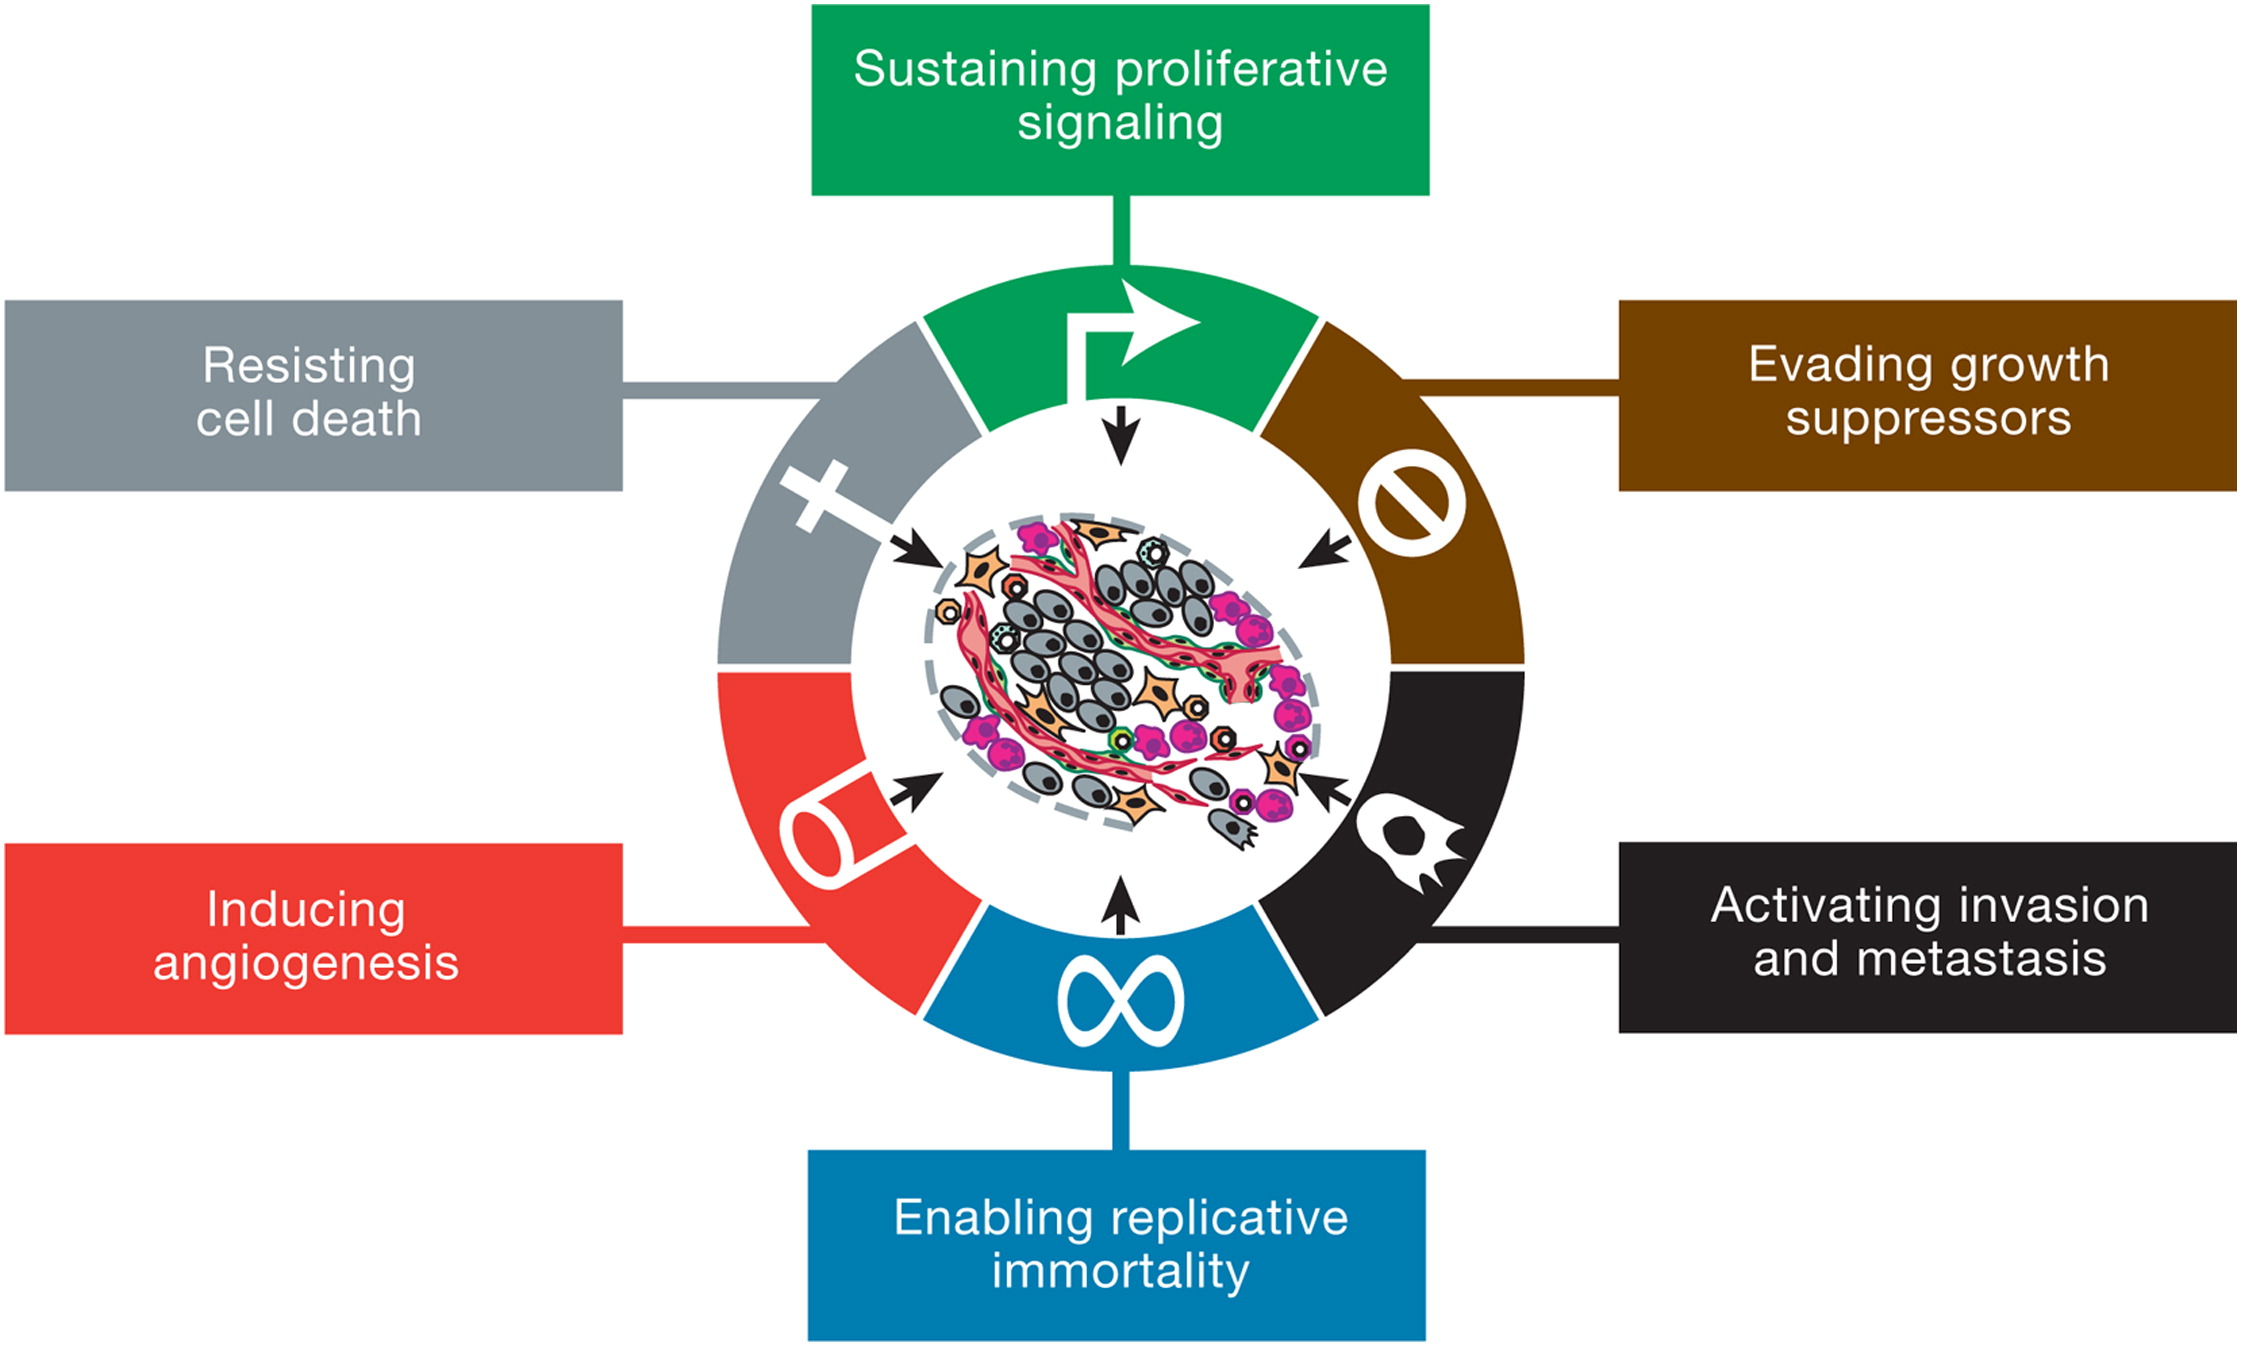
\includegraphics[width=.95\linewidth]{Figures/oldHallmarksCancer.jpg}
\caption[Original hallmarks of cancer]{Acquired capabilities of cancer; Functional capabilities acquired by most cancers during their development; Figure adapted from \protect\citeauthor*{Hanahan2000}\protect\cite{Hanahan2000}}\label{fig:oldhallmarks}
\end{figure}

However, with 11 years of additional research into the topic, more hallmarks have been found and the original list was revised by the authors to contain additional characteristics, namely 
\begin{enumerate*}
\item Avoiding immune destruction
\item Tumour-promoting inflamation
\item Genome instability and mutation
\item Deregulating cellular energetics
\end{enumerate*}
(\autoref{fig:newhallmarks}) \cite{Hanahan2011}. And even then a few years later, even more hallmarks e.g. metabolic rewiring are now considered a part of the characteristics of cancer \cite{Fouad2017}.

\begin{figure}[!ht]
\centering
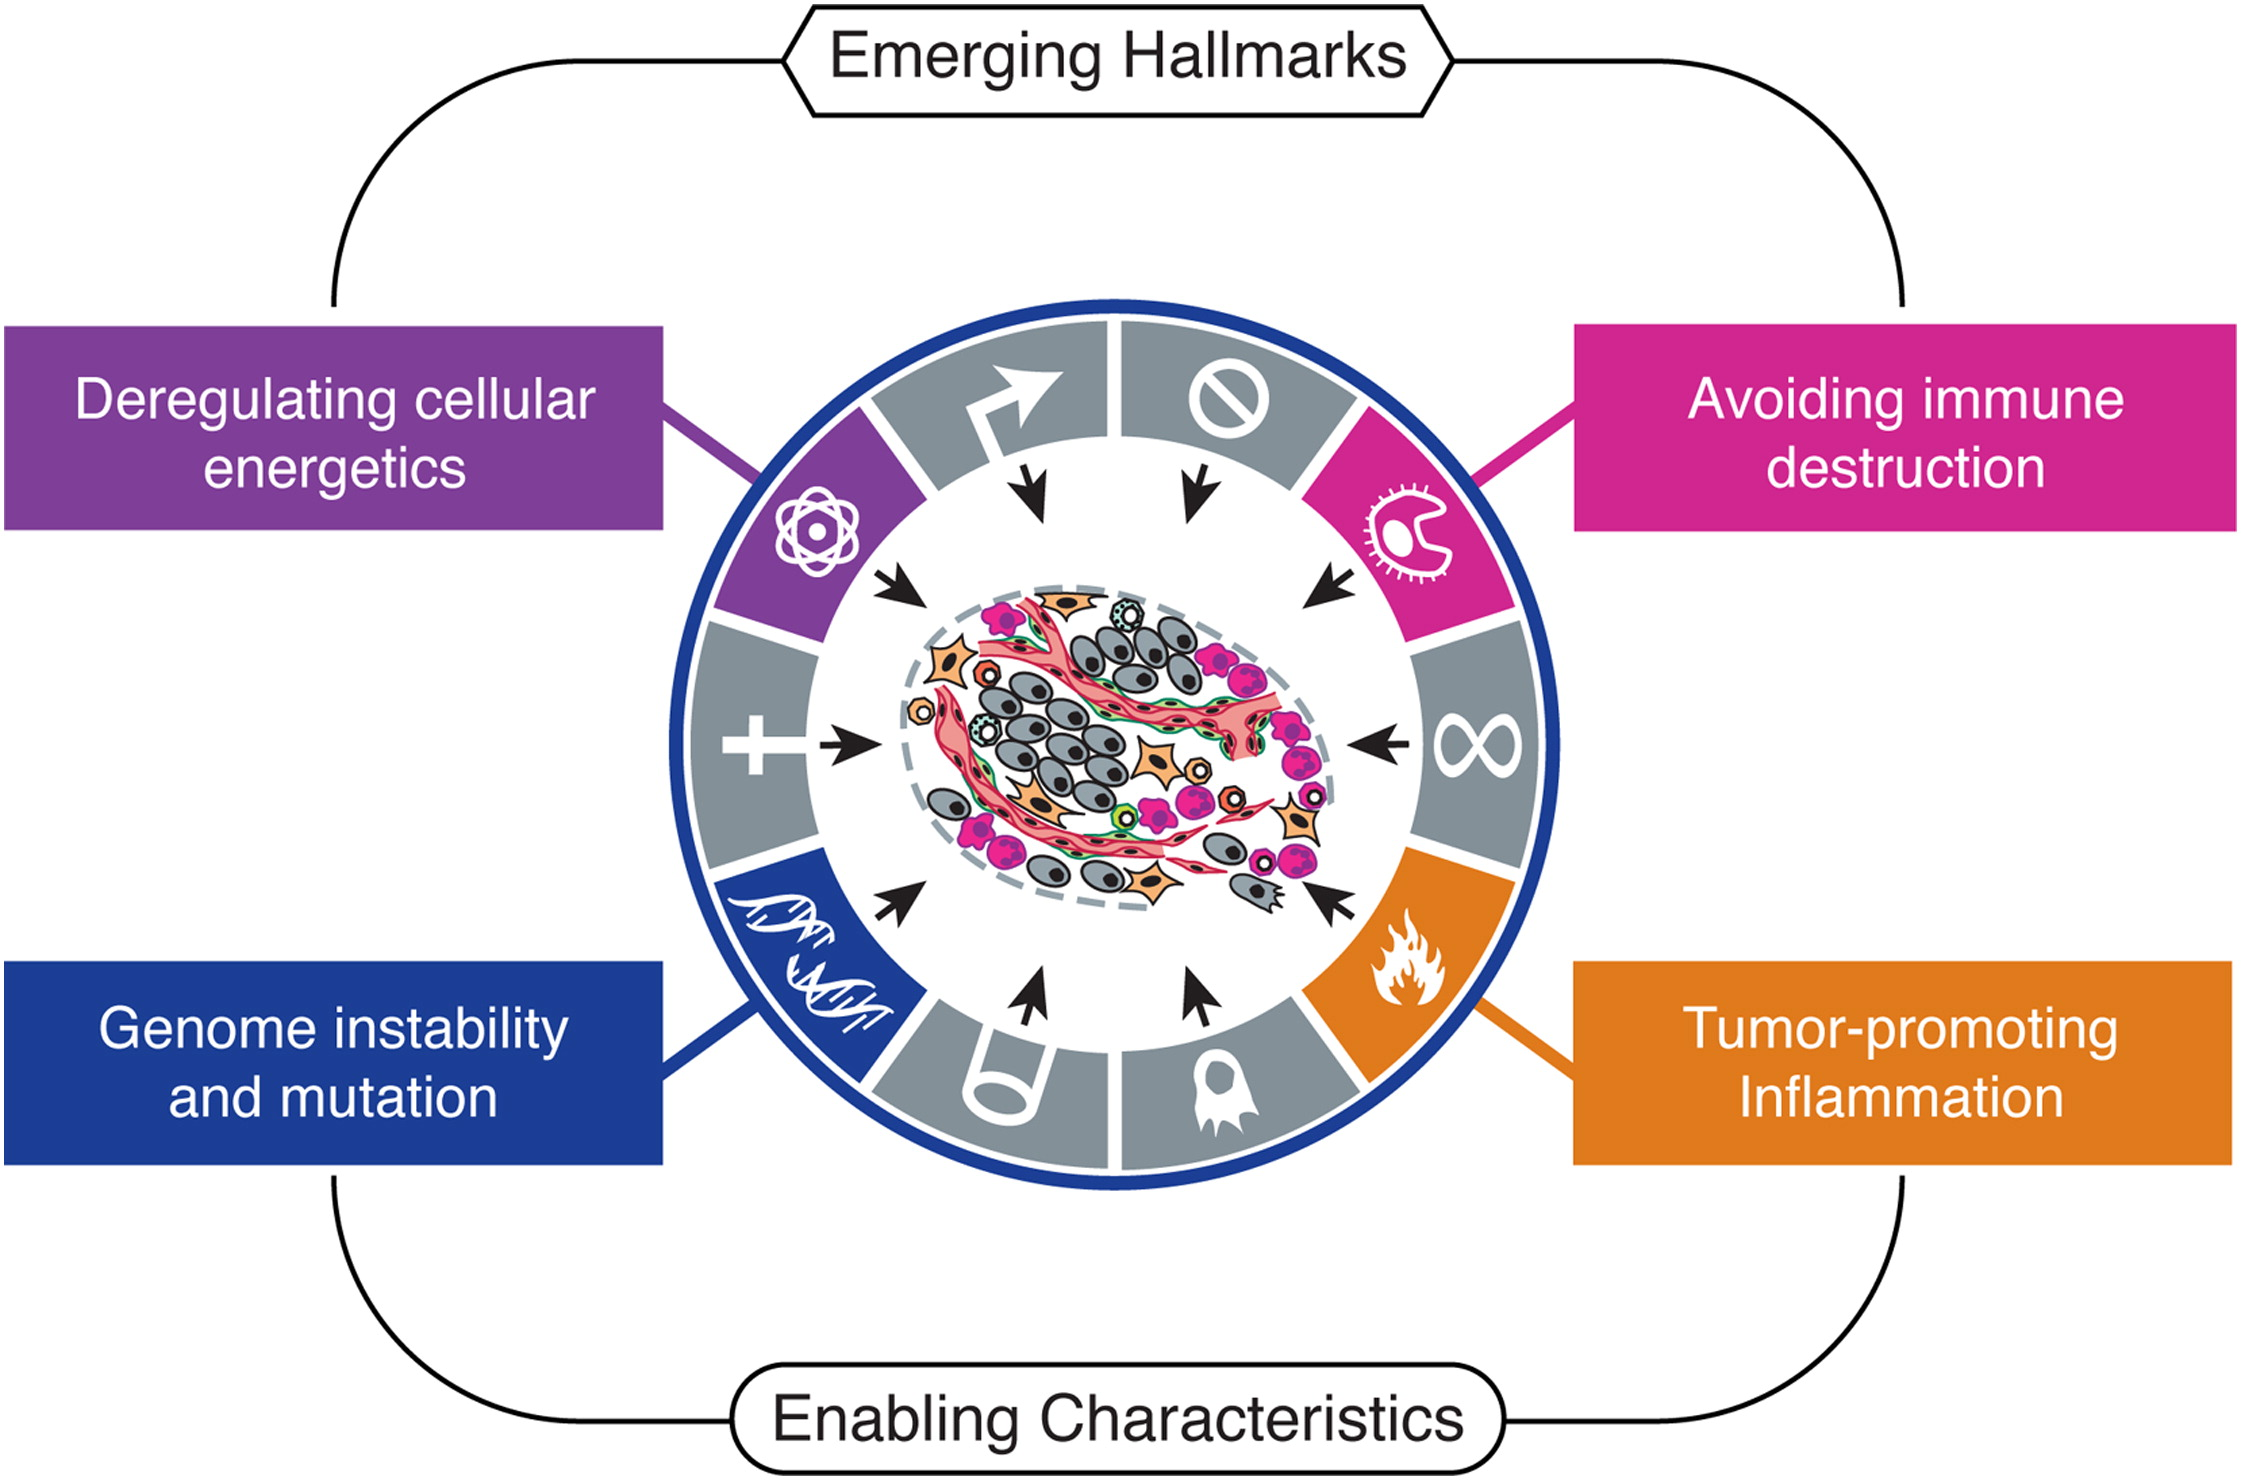
\includegraphics[width=.95\linewidth]{Figures/newHallmarksCancer.jpg}
\caption[New hallmarks of cancer]{Emerging hallmarks and enabling characteristics of cancer; updated version of the hallmarks figure (\autoref{fig:oldhallmarks}) with ; Figure adapted from \protect\citeauthor*{Hanahan2011}\protect\cite{Hanahan2011}}\label{fig:newhallmarks}
\end{figure}

So while the original set of the hallmarks was not sufficient or complete, it offered a good attempt at abstraction of biological concepts to describe cancers. In the following pages, I will outline each of those hallmarks and how it influences my research.

\todo[inline, color=red]{describe the hallmarks}

\subsubsection{Sustaining proliferative signaling - there are no breaks on the train}

\subsubsection{Evading growth suppressors}

\subsubsection{Activating invasion and metastasis - look at me... I am the organism now}

\subsubsection{Enabling replicative immortality}

\subsubsection{Inducing angiogenesis}

\subsubsection{Resisting cell death}

\subsection{Lungcancer}
\label{intro-sec:lungcancer}

With around 1.6 million deaths world-wide each year, lung cancer is the number one cause of cancer death \cite{Siegel2018}. Every year about twelve thousand Australians get diagnosed with lung cancer. These cases can be generally split into two groups: small cell lung cancers (SCLC) and non-small cell lung cancers (NSCLC), which account for around 15\% and 85\% of cases, respectively. The majority of NSCLC are either lung adenocarcinoma or lung squamous cell carcinoma \cite{Molina2008}. Even though smoking is highly associated with lung cancers, there is a big group of never smokers, with a high risk of lung cancers in East Asia, especially women, which is correlated with outside influences like pollution and occupational carcinogens and paired with genetic susceptibility \cite{Sun2007}.
This group usually shows \textit{EGFR} (epidermal growth factor receptor) driven tumours. EGFR is a transmembrane receptor tyrosine kinase, which is usually only expressed in epithelial, mesenchymal, and neurogenic tissue, but its overexpression in other tissues is a hallmark of many human malignancies, not just NSCLC.

\todo[inline]{Possibly change this to cancer in general}

%% original abstract
%Approximately 50% of patients with non-small cell lung cancer (NSCLC) develop acquired resistance to EGFR tyrosine kinase inhibitors (TKIs) through mutations in EGFR T790M. Maintaining a dynamic balance between T790M positive and negative clones offers an opportunity to delay the emergence of resistance and improve disease outcomes. It is now possible to quantify EGFR mutations using circulating tumour DNA (ctDNA) which can provide a surrogate measure of clonal populations within tumours. This project will utilise next generation sequencing (NGS) of tumour tissue and ctDNA in patients treated with EGFR TKIs to study clonal evolution patterns and predict optimal treatment approaches to delay therapeutic resistance.

% thesis overview
\section{Thesis overview and aims}
\label{intro-sec:overview}

While tumour heterogeneity is a well accepted concept by now, there is a need for computational methods assessing and visualising this heterogeneity. This work aims to contribute to this unmet need by developing three different custom made tools to infer and monitor tumour heterogeneity. I have completed the work in the following three parts:

\begin{enumerate}
	\item Development of two joint somatic variant calling workflows and the impact of these on downstream analysis (\autoref{ch:variantcalling}). 
	\item Analysis of five rapid autopsy probands with state of the art methods to investigate tumour heterogeneity and development of a mitochondrial based phylogeny reconstruction method (\autoref{ch:cascade}). 
	\item Development of a read-centric method to detect somatic mutational signatures from low coverage whole genome sequencing (\autoref{ch:mmf}).
\end{enumerate}
